\documentclass{ximera}

\input{../preamble.tex}

\title{4.2 - Logarithmic functions}


\begin{document}
\begin{abstract}

\end{abstract}
\maketitle

Logarithmic functions are designed to be the inverses of exponential functions. That is, 

\begin{definition}
  A \dfn{logarithmic function} is a function defined as follows
  \[
  \log_b(x) = y \qquad\text{means that}\qquad b^y = x
  \]
  where  $b\ne 1$ is a positive real number. The domain of a
  logarithmic function is $(0,\infty)$ and the range is $(- \infty, \infty)$.
\end{definition}

$b$ is called the \dfn{base}.

Remember that with exponential and logarithmic functions, there is one very special
base:
\[ e = 2.7182818284590\ldots \]
Since the exponential with base $e$,
$f(x) = e^x$ is often called the `natural exponential' functio,.  for the logarithm with base $e$,
we have a special notation, $\ln x$ is the `natural logarithm' function.  


\subsection{Connections between exponential functions and logarithms}

Let $b$ be a positive real number with $b\ne 1$.
\begin{itemize}
\item $b^{\log_b(x)} = x$ for all positive $x$
\item $\log_b(b^x) = x$ for all real $x$
\end{itemize}

\begin{question}
  What exponent makes the following expression true?
  \[
  3^x = e^{\left( x \cdot \answer{\ln 3} \right)}.
  \]
\end{question}


\section{Properties of logarithms}

Like exponential functions, and because they are inverse functions, logarithms also have useful properties. It's important to memorize these rules, as we will use them to make certain limits and derivatives easier (or possible in some situations!)

Let $b$ be a positive real number with $b\ne 1$.
\begin{itemize}
\item $\log_b(m\cdot n) = \log_b(m) + \log_b(n)$
\item $\log_b(m^n) = n\cdot \log_b(m)$
\item $\log_b\left(\frac{1}{m}\right) = \log_b(m^{-1}) = -\log_b(m)$
\item $\log_a(m) = \frac{\log_b(m)}{\log_b(a)}$
\end{itemize}

\begin{question}
  What value makes the following expression true?
  \[
  \log_2\left(\frac{8}{16}\right) = 3-\answer{4}
  \]
\end{question}


\begin{question}
  What makes the following expression true?
  \[
  \log_3(x) = \frac{\ln(x)}{\answer{\ln(3)}}
  \]
\end{question}


\section{Exponential equations}
Let's look into solving equations involving these functions.  We'll start with a straightforward example.
\begin{example}
	Solve the equation: $\displaystyle 4^x = 8$.
	\begin{explanation}
		We know $4$ and $8$ are each powers of $2$, we start by rewriting in terms of this base.
		\[ 4^x = 2^{2x}  \,\,\, \textrm{ and } \,\,\, 8 =2^{\answer{3}} \,\,\,\, \textrm{ so } 2^{2x} = 2^{\answer{3}} \]
		Since exponential functions are one-to-one, the only way for $a^m = a^n$ is if $m=n$.  In this case,
		that means $\displaystyle 2x = 3$.
		
		The solution is: $\displaystyle x = \answer{3/2}$.
	\end{explanation}
\end{example}


Of course, if we couldn't rewrite both sides with the same base, we can still use the properties of logarithms to solve.
\begin{example}
	Solve the equation: $\displaystyle 5^{2x-3} = 7$.
	\begin{explanation}
		Since we can't easily rewrite both sides as exponentials with the same base, we'll use logarithms instead.  Above we said that
		$\log_b(x) = y$ means that $b^y = x$.  That statement means that each exponential equation has an equivalent logarithmic form
		and vice-versa.  We'll convert to a logarithmic equation and solve from there.
		\begin{align*}
			5^{2x-3} &= 7\\
			\log_{\answer{5}}\left(  \answer{7} \right) &= 2x-3
		\end{align*}
		From here, we can solve for $x$ directly.
		\begin{align*}
			2x &= \log_{5}\left(7\right) + 3\\
			x &= \frac{\log_{5}\left(7\right) + 3}{2}
		\end{align*}
	\end{explanation} 
\end{example}


\begin{example}
	Solve the equation: $\displaystyle e^{2x} = e^x + 6$. 
	\begin{explanation}
		Immediately taking logarithms of both sides will not help here, as the right side has multiple terms.  We know that logarithms do not
		behave well with sums, but with products/quotients.  Instead, we notice that $e^{2x} = \left(e^x\right)^2$. (This is a common trick that
		you will likely see many times.)  
		\begin{align*}
			e^{2x} &= e^x + 6\\
			\left(e^x\right)^2 &= e^x + 6\\
			\left(e^x\right)^2 - e^x - 6 &= 0
		\end{align*}
		Our equation is really a quadratic equation in $e^x$!  The left-hand side factors as $\left( e^x - \answer{3}\right) \left(e^x + \answer{2}\right)$, so we are dealing
		with \[ e^x - \answer{3} = 0  \qquad  \textrm{and} \qquad e^x+\answer{2} = 0.\]
		For the first:
		\begin{align*}
			e^x &= \answer{3}\\
			x &= \ln\left( \answer{3}\right).
		\end{align*}
		
		From the second: $\displaystyle e^x = \answer{-2}$.  Look back at the graph of $y=e^x$ above.  What was the range of the exponential function?  It didn't include any negative
		numbers, so $e^x = -2$ has no solutions. 
		
		The solution to $\displaystyle e^{2x} = e^x + 6$ is $x = \answer{\ln(3)}$.
	\end{explanation}
\end{example}

\begin{problem}
	Solve the equation: $\displaystyle 2\left(5^{2x} + 6\right) = 11 \cdot 5^x$.
	\begin{selectAll}
		\choice[correct]{$\displaystyle \log_{5}\left(\dfrac{3}{2} \right)$}
		\choice{$\displaystyle \frac{\ln\left(\dfrac{3}{2} \right)}{5}$}
		\choice{$\displaystyle \log_{4}\left(5\right)$}
		\choice[correct]{$\displaystyle \log_{5}\left(4 \right)$}
		\choice{The equation has no solutions.}
	\end{selectAll}
\end{problem}

\begin{example}
	Solve the inequality: $\displaystyle \frac{6^x - 7 \cdot 3^x}{4^x - 15} \ge 0$.
	\begin{explanation}
		Since this isn't a linear inequality, we'll solve it using a sign-chart.  Luckily, the right-side is already $0$.  Let's factor the numerator on the left:
		\begin{align*} 
			6^x - 7 \cdot 3^x &= \left(2\cdot 3\right)^x - 7 \cdot 3^x \\
				&= 2^x \cdot 3^x - 7 \cdot 3^x\\
				&= 3^x \left( 2^x - 7 \right).
		\end{align*}
		That means we need to construct a sign chart for $\displaystyle \frac{3^x \left( 2^x - 7\right)}{4^x - 15}$.
		(Note: $\log_{2}(7)$ is about $2.81$ and $\log_{4}(15)$ is about $1.95$.)
		
		\begin{center}
		\begin{tikzpicture} 
			\tkzTabInit[lgt=2,espcl=1] 
				{$x$         /1, 
				$3^x$   /1, 
				$2^x-7$  /1,
				$4^x-15$       /1}% 
				{  , $\log_{4}(15)$ \,\,\,\,\, , \,\,\,\,\,\,$\log_{2}(7)$ ,  }% 
			\tkzTabLine{ , + , d , +  , t , + ,}
			\tkzTabLine{ , - , d , - , t , + ,}
			\tkzTabLine{ , - , d ,  + , t , +, }
		\end{tikzpicture} 
		\end{center}
		The solution is:
		\[ \left( -\infty, \, \log_{4}(15) \, \right) \bigcup \left[ \,\log_{2}(7) \,, \infty \right) \]
	\end{explanation}
\end{example}
\section{Logarithmic equations}

\begin{example}
	Solve the equation: $\displaystyle \log_5( 2x+1) = 3$.
	\begin{explanation}
		Our first step will be to rewrite this logarithmic equation into its exponential form.
		\[ \log_5(2x+1) = 3 \qquad \textrm{ means } \qquad 2x+1 = 5^{\answer{3}} \]
		From here we solve directly.
		\begin{align*}
			2x+1 &= \answer{125}\\
			2x &= \answer{124}\\
			x &= \answer{62}.
		\end{align*}
	\end{explanation}
\end{example}



\begin{example}
	Solve the equation: \[ \log_3(2x+1) = 1-\log_3(x+2). \]
	\begin{explanation}
		With more than one logarithm, we'll typically try to use the properties of logarithms to combine them into a single term.
		\begin{align*}
			\log_3(2x+1) &= 1-\log_3(x+2) \\
			\log_3(2x+1) + \log_3(x+2) &= 1\\
			\log_3\left( (2x+1)(x+2)\right) &= 1\\
			\log_3\left( 2x^2 + 5x + 2 \right) &= 1\\
			2x^2 + 5x + 2 &= 3\\
			2x^2 + 5x - 1 &= 0
		\end{align*}
		Let's use quadratic formula to solve this.
		\[ x = \frac{-5 \pm \sqrt{5^2 - 4 \cdot 2\cdot -1}}{2 \cdot 2} = \frac{ -5\pm \sqrt{ \answer{33} } }{4}. \]
		
		What happens if we try to plug $x = \dfrac{-5 - \sqrt{33}}{4}$ into the equation?  Both $2\left( \dfrac{-5-\sqrt{33}}{4} \right) + 1$ and $\dfrac{-5-\sqrt{33}}{4} + 2$ are 
		negative.  That means, the logarithms of these values is not defined.  
		
		It turns out that $\dfrac{-5 - \sqrt{33}}{4}$ is a solution of the equation $2x^2+5x-1 = 0$,
		but not a solution of the original equation $\log_3(2x+1) = 1-\log_3(x+2)$. 
		
		When working with logarithmic equations, we must always check that the solutions we find 
		actually satisfy the original equation.
		
		The only solution is $x = \dfrac{-5 + \sqrt{33}}{4}$.
		
	\end{explanation}		
\end{example}





\end{document}